% !TeX program = pdflatex
% =============================================================
% Public Economics -- Research Designs for Causal Inference
% English adaptation of "Forschungsdesigns: Daten und Forschungsdesigns
% in der Oekonomie" by Alexander Ahammer (Department of Economics,
% Johannes Kepler University Linz), version 1 December 2025.
% Translated and adapted for WU Vienna. Figures reproduced from
% external papers in the original are left as placeholders (see
% \figplaceholder calls below) pending permission/source files;
% the author's own illustrative diagrams and simulated-data examples
% are redrawn natively in TikZ.
% =============================================================
\documentclass[11pt,aspectratio=169]{beamer}

\usetheme{metropolis}
\usepackage[utf8]{inputenc}
\usepackage[T1]{fontenc}
\usepackage{lmodern}
\usepackage{booktabs}
\usepackage{array}
\usepackage{textcomp}
\usepackage{siunitx}
\usepackage{tikz}
\usepackage{pgfplots}
\pgfplotsset{compat=1.18}
\usepackage{eso-pic}
\usetikzlibrary{positioning,arrows.meta,calc}

% ----------------------------------------------------------------
% Colors: WU Vienna blue as primary accent
% ----------------------------------------------------------------
\definecolor{wublue}{HTML}{003D7C}
\definecolor{wulight}{HTML}{4F8FC4}
\definecolor{wugray}{HTML}{5C6670}
\definecolor{wured}{HTML}{B0202E}
\definecolor{wugreen}{HTML}{4C8C6B}
\definecolor{wuyellow}{HTML}{D9A441}
\setbeamercolor{palette primary}{bg=wublue,fg=white}
\setbeamercolor{frametitle}{bg=wublue,fg=white}
\setbeamercolor{progress bar}{fg=wublue,bg=wulight!30}
\setbeamercolor{alerted text}{fg=wured}

\setbeamertemplate{frame footer}{Research Designs}
\setbeamertemplate{footline}[frame number]

\title{Public Economics}
\subtitle{Research Designs for Causal Inference}
\author{Shushanik Margaryan}
\institute{WU Vienna University of Economics and Business}
\date{Winter Term}

% Source note command for footnote-style citations on data slides
\newcommand{\srcnote}[1]{{\footnotesize\color{wugray}Source: #1}}

% Placeholder box for figures reproduced from external sources
% #1 = width (cm), #2 = height (cm), #3 = caption/description text
\newcommand{\figplaceholder}[3]{%
  \begin{center}
  \begin{tikzpicture}
    \draw[wugray, thick, dash pattern=on 4pt off 3pt, fill=wugray!7] (0,0) rectangle (#1,#2);
    \draw[wugray, thin] (0,0) -- (#1,#2); \draw[wugray, thin] (0,#2) -- (#1,0);
    \node[align=center, text width=#1 cm-1.2cm, wugray] at (#1/2,#2/2) {\footnotesize\itshape FIGURE PLACEHOLDER\\[2pt] #3};
  \end{tikzpicture}
  \end{center}
}

\titlegraphic{
\includegraphics[height=1.0cm]{../assets/wu_logo.png}}

\begin{document}

% =============================================================
\begin{frame}
  \titlepage
\end{frame}

\AddToShipoutPictureFG{%
  \AtPageUpperLeft{%
    \put(\LenToUnit{\paperwidth-2.0cm},\LenToUnit{-0.85cm}){
\includegraphics[height=0.62cm]{../assets/wu_logo_white.png}}%
  }%
}

\begin{frame}{Acknowledgment}
  \begin{block}{Credit}
    This lecture is based on teaching material originally developed by \textbf{Alexander Ahammer} (Department of Economics, Johannes Kepler University Linz), from his course slides \emph{``Forschungsdesigns: Daten und Forschungsdesigns in der \"Okonomie''} (version 1 December 2025).
  \end{block}
  \vspace{0.5em}
  \begin{itemize}
    \item Translated from German to English and lightly adapted for WU Vienna.
    \item Figures reproduced from external papers in the original slides are marked as placeholders here, pending the original image files.
    \item All illustrative diagrams and simulated-data examples are redrawn to match this course's visual style.
  \end{itemize}
\end{frame}

% =============================================================
\begin{frame}{Agenda}
  \tableofcontents
\end{frame}

% =============================================================
\section{Experiments}

\begin{frame}{Experiments}
  \begin{itemize}
    \item We have seen that experiments (randomized control trials, RCTs) can solve the fundamental problem of causal inference.
    \item RCTs are the gold standard of causal inference.
    \item In the social sciences, RCTs are often difficult to implement:
    \begin{itemize}
      \item A double-blind protocol is typically not possible
      \item Too expensive
      \item Conceptually possible but not practically feasible
      \item Ethical concerns
      \item Fairness
    \end{itemize}
    \vspace{0.3em}
    \item Nonetheless, they are used increasingly often:
    \begin{itemize}
      \item Social experiments for policy evaluation
      \item Lab experiments in behavioral economics
      \item Field experiments in development and labor economics
      \item Increasingly common in other fields too
    \end{itemize}
  \end{itemize}
\end{frame}

\begin{frame}{Experiments}
  \framesubtitle{Example 1: RAND Health Insurance Experiment}
  \begin{itemize}
    \item How does cost-sharing (coinsurance/copayments) in health insurance affect health care spending?
    \item 1974--1981, $\sim$5{,}800 randomly selected people (representative of the US population under 62) receive health insurance with a variable deductible/coinsurance rate.
    \item Cost: \$295 million; data collected mostly via surveys.
    \item Enormous influence on policy and the insurance industry.
  \end{itemize}
\end{frame}

\begin{frame}{Coinsurance Rates vs.\ the Free Care Plan}
  \figplaceholder{11}{5.3}{Aron-Dine et al.\ (2013), Table 2: ``Plans' Effects on Utilization'' --- spending and utilization by coinsurance arm (0\%, 25\%, mixed, 50\%, individual deductible, 95\%)}
  \srcnote{Aron-Dine, Einav \& Finkelstein (2013), \emph{Journal of Economic Perspectives} 27(1).}
\end{frame}

\begin{frame}{Experiments}
  \framesubtitle{Example 2: Monetary Incentives in the Workplace}
  \begin{itemize}
    \item Classic management problem: when monitoring is difficult or impossible, how can productivity best be maximized through incentive schemes?
    \item Does pay-for-performance (PFP) increase the productivity of existing employees (\emph{incentive effect}) and attract more productive new employees (\emph{selection effect})?
    \begin{itemize}
      \item PFP raises the marginal product of an extra unit of effort for the employee.
    \end{itemize}
    \item Can we compare firms with different incentive schemes? No --- these schemes are endogenous to firm success.
    \item We need experimental variation, ideally \emph{within} a single firm.
  \end{itemize}
\end{frame}

\begin{frame}{Experiments}
  \framesubtitle{Example 2: Monetary Incentives in the Workplace}
  \begin{itemize}
    \item \textbf{Shearer (2004)}
    \item Tree planters in British Columbia (Canada), randomly assigned to fixed-wage vs.\ piece-rate pay on each workday.
    \item \textbf{Incentive effect}: 20\% productivity gain on piece-rate days.
    \item But higher variance in productivity.
    \item No evidence of a selection effect.
  \end{itemize}
\end{frame}

\begin{frame}{Experiments}
  \framesubtitle{Example 3: Moving to Opportunity (MTO)}
  \begin{itemize}
    \item How important is neighborhood/environment for economic outcomes? A randomized mobility experiment.
    \item 4{,}600 low-income families with children, since 1994.
    \begin{itemize}
      \item \textbf{Treatment}: housing vouchers for low-poverty areas, plus counseling.
      \item \textbf{Control}: no vouchers.
    \end{itemize}
    \item \textbf{Results}: better housing, few short-run effects --- education unchanged, labor-market effects unclear.
    \item \textbf{Chetty et al.\ (2016)}: matched with tax data, long-run effects on children --- college attendance $\uparrow$, income $\uparrow$, single parenthood $\downarrow$.
    \item \url{http://www2.nber.org/mtopublic/}
  \end{itemize}
\end{frame}

\begin{frame}{Experiments}
  \framesubtitle{Example 4: Welfare Effects of Social Media}
  \begin{itemize}
    \item Social media has potential costs and benefits.
    \begin{itemize}
      \item \textbf{Benefits}: lower cost of connecting, communicating, and sharing information.
      \item \textbf{Costs}: negative correlations with mental health, cyberbullying, political polarization.
    \end{itemize}
    \item \textbf{Allcott et al.\ (2020, AER)}: RCT with 2{,}743 Facebook users, before the 2018 midterm elections; the treatment group was paid to deactivate their account.
    \item \textbf{Results}:
    \begin{itemize}
      \item Less online activity, more TV watching and social activities
      \item Less ``news knowledge'' and political polarization
      \item Higher subjective well-being
      \item Long-lasting reduction in Facebook use
    \end{itemize}
  \end{itemize}
\end{frame}

\begin{frame}{Econometric Analysis of Experiments}
  \begin{itemize}
    \item With experiments, the workload is highest \emph{before} the first results are available.
    \item Analysis of experimental data is relatively simple.
    \item If randomization worked, comparing means between the treatment and control group is sufficient.
    \item OLS regressions can control for additional variables:
  \end{itemize}
  \[
    Y_i = \beta_0 + \beta_1 D_i + \gamma X + \varepsilon_i \tag{1}
  \]
\end{frame}

\begin{frame}{Potential Problems with Experiments}
  \begin{itemize}
    \item \textbf{Non-random assignment}
    \begin{itemize}
      \item Test baseline characteristics between treatment ($T$) and control ($C$) groups
    \end{itemize}
    \item \textbf{Non-compliance}
    \begin{itemize}
      \item $C$ also gets treated
      \item $T$ does not take up the treatment
    \end{itemize}
    \item \textbf{Attrition}
    \begin{itemize}
      \item Participants leave the experiment
    \end{itemize}
    \item \textbf{Hawthorne effect / experimenter demand effects}
    \begin{itemize}
      \item Participants behave differently because they know they are part of an experiment
    \end{itemize}
  \end{itemize}
\end{frame}

% =============================================================
\section{Natural Experiments}

\begin{frame}{Natural Experiments}
  \begin{itemize}
    \item We are often interested in questions that cannot be answered through experiments.
    \item In (non-experimental) observational data, this is possible --- but we need a \textbf{design}.
    \item We primarily look for so-called \textbf{natural experiments}.
    \begin{itemize}
      \item Synonyms: quasi-experiments, accidental experiments
    \end{itemize}
    \item Natural experiments are circumstances that cause otherwise identical people to receive a treatment quasi-randomly, while others do not:
    \begin{itemize}
      \item Nature (e.g.\ weather, multiple births, health shocks)
      \item (Arbitrary) administrative rules (e.g.\ Maimonides' rule, age cutoffs)
      \item (Unpredictable) changes in law (e.g.\ minimum wages)
      \item Geographic variation/boundaries (e.g.\ broadband internet access)
      \item Natural disasters
    \end{itemize}
  \end{itemize}
\end{frame}

\begin{frame}{Natural Experiments}
  \begin{itemize}
    \item To analyze natural experiments, we need additional econometric methods:
    \begin{itemize}
      \item Event studies
      \item Difference-in-differences
      \item Instrumental variables
      \item Regression discontinuity designs
    \end{itemize}
  \end{itemize}
  \vspace{0.5em}
  \begin{alertblock}{Trade-off}
    \textbf{Pros}: cheap to carry out. \textbf{Cons}: hard to find, external validity concerns.
  \end{alertblock}
\end{frame}

% =============================================================
\section{Event Studies}

\begin{frame}{Event Studies}
  \begin{itemize}
    \item \textbf{Setting}: we have an outcome $y$ that varies over time.
    \begin{itemize}
      \item Time-series or panel data required.
    \end{itemize}
    \item Treatment occurs at time $t=0$ (e.g.\ a policy change).
    \item \textbf{Idea}: everything that happens before $t=0$ is unrelated to the treatment. Everything that happens after $t=0$ is conditioned on the treatment.
    \item If the outcome trend is ``flat'' before $t=0$, we can make an assumption about the counterfactual:
    \begin{itemize}
      \item How would the trend have evolved \emph{without} the treatment?
    \end{itemize}
  \end{itemize}
\end{frame}

\begin{frame}{Event Studies}
  \centering
  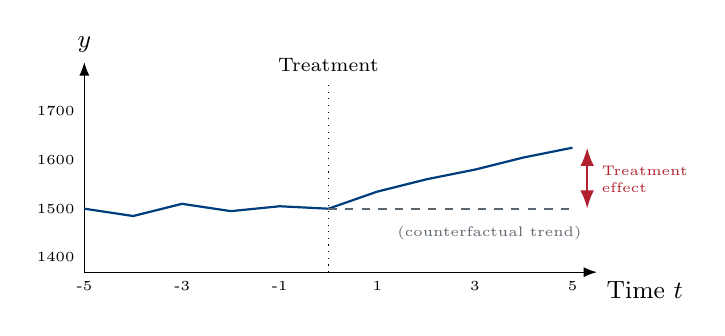
\begin{tikzpicture}[scale=0.62]
    \draw[-{Latex}] (0,-0.3) -- (10.5,-0.3) node[below right, font=\small]{Time $t$};
    \draw[-{Latex}] (0,-0.3) -- (0,4) node[above, font=\small]{$y$};
    \foreach \t/\lab in {0/-5,2/-3,4/-1,6/1,8/3,10/5}
      \node[below, font=\tiny] at (\t,-0.3) {\lab};
    \foreach \val/\lab in {0/1400,1/1500,2/1600,3/1700}
      \node[left, font=\tiny] at (0,\val) {\lab};
    \draw[dotted] (5,-0.3) -- (5,3.6);
    \node[above, font=\scriptsize] at (5,3.6) {Treatment};
    % raw trend: flat pre, rising post
    \draw[wublue, thick] plot coordinates {(0,1.00) (1,0.85) (2,1.10) (3,0.95) (4,1.05) (5,1.00)};
    \draw[wublue, thick] plot coordinates {(5,1.00) (6,1.35) (7,1.60) (8,1.80) (9,2.05) (10,2.25)};
    % counterfactual (stage 2+)
    \onslide<2->{
      \draw[wugray, thick, dashed] (5,1.00) -- (10,1.00);
      \node[below, font=\tiny, wugray] at (8.3,0.85) {(counterfactual trend)};
    }
    % treatment effect arrow (stage 3+)
    \onslide<3->{
      \draw[wured, thick, {Latex}-{Latex}] (10.3,1.00) -- (10.3,2.25);
      \node[right, font=\tiny, wured, align=left] at (10.4,1.6) {Treatment\\ effect};
    }
  \end{tikzpicture}
\end{frame}

\begin{frame}{Event Studies}
  \begin{itemize}
    \item The counterfactual trend is an \textbf{assumption}.
    \begin{itemize}
      \item Not testable $\longrightarrow$ the fundamental problem of causal inference.
    \end{itemize}
    \item If we are willing to assume that, absent treatment, the trend would have simply continued, the difference between the blue and gray lines is the treatment effect.
    \item Another important assumption: nothing \emph{else} may happen at $t=0$ that could affect the outcome.
    \begin{itemize}
      \item Must be argued for.
      \item Requires institutional knowledge.
    \end{itemize}
  \end{itemize}
\end{frame}

\begin{frame}{Event Studies}
  Estimation with a simple OLS regression:
  \[
    y_{it} = \beta_0 + \delta\, post_{it} + \varepsilon_{it} \tag{2}
  \]
  \begin{itemize}
    \item $post_{it}$ is a dummy variable equal to 1 in every period $t > 0$ and 0 in prior periods.
    \item $\delta$ is the treatment effect (the difference in $y$-means between the pre- and post-treatment period).
  \end{itemize}
\end{frame}

\begin{frame}{Event Studies}
  If we are interested in \textbf{dynamic effects}, estimate with period dummies:
  \[
    y_{it} = \beta_0 + \delta_{-5} t_{i,-5} + \delta_{-4} t_{i,-4} + \dots + \delta_{-1} t_{i,-1} + \delta_1 t_{i,1} + \delta_2 t_{i,2} + \dots + \delta_5 t_{i,5} + \varepsilon_{it}
  \]
  \[
    = \beta_0 + \sum_{k=-5 \,|\, k \neq 0}^{5} \delta_k t_{ik} + \varepsilon_{it} \tag{3}
  \]
  \begin{itemize}
    \item We define $t_0$ as the base period and therefore omit its dummy.
    \item The coefficients $\hat\delta_k$ measure the difference between $y_k$ in each period $k$ and $y_0$ at $t=0$.
  \end{itemize}
\end{frame}

\begin{frame}[fragile]
  \frametitle{Simulated Example: The Data}
{\scriptsize
\begin{verbatim}
. list id t post y in 1/22, sepby(id)

       id      t      post         y

 1.     1    -5         0    1500.392
 2.     1    -4         0    1458.272
 3.     1    -3         0    1668.017
 4.     1    -2         0    1546.392
 5.     1    -1         0    1425.803
 6.     1     0         0    1533.735
 7.     1     1         1     1492.77
 8.     1     2         1    1618.688
 9.     1     3         1    1635.518
10.     1     4         1    1582.649
11.     1     5         1    1682.446

   [... id 2 omitted here, same structure ...]
\end{verbatim}
}
\end{frame}

\begin{frame}[fragile]
  \frametitle{Simulated Example: Simple Mean Comparison}
{\scriptsize
\begin{verbatim}
. ttest y, by(post)
Two-sample t test with equal variances

   Group        Obs        Mean   Std. Err.   Std. Dev.    [95% Conf. Interval]

       0      6,000   1498.789     1.04265    80.76335     1496.746   1500.833
       1      5,000   1576.126    1.227076    86.76741     1573.721   1578.532

combined    11,000     1533.943   .8770979    91.99081     1532.223   1535.662

    diff              -77.33677   1.599783                -80.47264   -74.20091

    diff = mean(0) - mean(1)                                       t = -48.3421
Ho: diff = 0                                      degrees of freedom =    10998
Ha: diff < 0                  Ha: diff != 0                 Ha: diff > 0
Pr(T < t) = 0.0000          Pr(|T| > |t|) = 0.0000          Pr(T > t) = 1.0000
\end{verbatim}
}
\end{frame}

\begin{frame}[fragile]
  \frametitle{Simulated Example: Equation (2) by OLS}
{\scriptsize
\begin{verbatim}
. reg y post
      Source            SS            df         MS        Number of obs    =    11,000
                                                            F(1, 10998)      =   2336.95
       Model     16311754.6            1    16311754.6     Prob > F         =    0.0000
    Residual     76765177.5       10,998    6979.92158     R-squared        =    0.1753
                                                            Adj R-squared    =    0.1752
       Total     93076932.1       10,999    8462.30858     Root MSE         =    83.546

           y           Coef.    Std. Err.        t       P>|t|     [95% Conf. Interval]

        post         77.33677   1.599783      48.34      0.000     74.20091       80.47264
       _cons         1498.789   1.078573    1389.60      0.000     1496.675       1500.904
\end{verbatim}
}
\vspace{0.3em}
$\Rightarrow$ Without control variables, the OLS estimator equals the difference in means between the pre- and post-treatment period.\\
$\Rightarrow$ The estimated treatment effect is \textbf{77.3}.
\end{frame}

\begin{frame}[fragile]
  \frametitle{Simulated Example: Period Dummies}
{\scriptsize
\begin{verbatim}
. quietly tabulate t, gen(dt_)
. list id t dt_* in 1/22, sepby(id)

       id     t       dt_1   dt_2   dt_3   dt_4   dt_5   dt_6   dt_7   dt_8   dt_9  dt_10  dt_11

 1.     1    -5         1      0      0      0      0      0      0      0      0      0      0
 2.     1    -4         0      1      0      0      0      0      0      0      0      0      0
 3.     1    -3         0      0      1      0      0      0      0      0      0      0      0
 4.     1    -2         0      0      0      1      0      0      0      0      0      0      0
 5.     1    -1         0      0      0      0      1      0      0      0      0      0      0
 6.     1     0         0      0      0      0      0      1      0      0      0      0      0
 7.     1     1         0      0      0      0      0      0      1      0      0      0      0
 8.     1     2         0      0      0      0      0      0      0      1      0      0      0
 9.     1     3         0      0      0      0      0      0      0      0      1      0      0
10.     1     4         0      0      0      0      0      0      0      0      0      1      0
11.     1     5         0      0      0      0      0      0      0      0      0      0      1
\end{verbatim}
}
\end{frame}

\begin{frame}[fragile]
  \frametitle{Simulated Example: Equation (3) by OLS}
{\tiny
\begin{verbatim}
. reg y dt_1-dt_5 dt_7-dt_11
      Source         SS               df         MS        Number of obs      =     11,000
                                                            F(10, 10989)       =     343.21
      Model      22151716.7           10    2215171.67     Prob > F           =     0.0000
   Residual      70925215.4       10,989    6454.20105     R-squared          =     0.2380
                                                            Adj R-squared      =     0.2373
      Total      93076932.1       10,999    8462.30858     Root MSE           =     80.338

           y           Coef.    Std. Err.        t       P>|t|       [95% Conf. Interval]

       dt_1          5.825865   3.592826       1.62   0.105         -1.216721       12.86845
       dt_2          2.872052   3.592826       0.80   0.424         -4.170535       9.914638
       dt_3          5.407958   3.592826       1.51   0.132         -1.634629       12.45054
       dt_4          2.766989   3.592826       0.77   0.441         -4.275597       9.809575
       dt_5          5.954441   3.592826       1.66   0.097         -1.088145       12.99703
       dt_7          35.16286   3.592826       9.79   0.000          28.12027       42.20544
       dt_8          54.08144   3.592826      15.05   0.000          47.03886       61.12403
       dt_9          80.86031   3.592826      22.51   0.000          73.81772       87.90289
      dt_10          106.0099   3.592826      29.51   0.000          98.96728       113.0524
      dt_11          129.5922   3.592826      36.07   0.000          122.5496       136.6347
      _cons          1494.985   2.540512     588.46   0.000          1490.005       1499.965
\end{verbatim}
}
\end{frame}

\begin{frame}{The Dynamic Coefficients, Plotted}
  \centering
  \begin{tikzpicture}[scale=0.62]
    \draw[-{Latex}] (0,0) -- (10.5,0) node[below right, font=\small]{Time $t$};
    \draw[-{Latex}] (0,-0.6) -- (0,4.2) node[above, font=\small]{OLS estimate};
    \foreach \t/\lab in {0/-5,2/-3,4/-1,6/1,8/3,10/5}
      \node[below, font=\tiny] at (\t,0) {\lab};
    \foreach \val/\lab in {-0.5/-25,0/0,1/25,2/50,3/75,4/100,4.6/125}
      \node[left, font=\tiny] at (0,\val) {\lab};
    \draw[dotted] (0,0) -- (10,0);
    % coefficients: dt_1..dt_5 at t=-5..-1, 0 at t=0, dt_7..dt_11 at t=1..5
    \foreach \x/\y in {0/0.117, 2/0.057, 4/0.108, 6/0.055, 8/0.119, 10/0}
      \fill[wublue] (\x,\y) circle (2.2pt);
    \fill[wublue] (5,0) circle (2.2pt);
    \foreach \x/\y in {6/0.703, 7/1.082, 8/1.617, 9/2.120, 10/2.592}
      \fill[wured] (\x,\y) circle (2.2pt);
  \end{tikzpicture}
  \vspace{0.3em}
  \footnotesize Coefficients from the regression on the previous slide: flat and insignificant before treatment ($t<0$), rising sharply and significantly after ($t>0$).
\end{frame}

\begin{frame}{Event Studies}
  \framesubtitle{Example 1: Children}
  \figplaceholder{11}{5.3}{Kleven et al.\ (2019) --- event-study plots of earnings and hours worked relative to first childbirth, by gender (``child penalty'')}
  \srcnote{Kleven, Landais \& S{\o}gaard (2019), \emph{AEJ: Applied Economics} 11(4).}
\end{frame}

\begin{frame}{Event Studies}
  \framesubtitle{Example 2: The Heroin Epidemic}
  \figplaceholder{11}{5.3}{Evans, Lieber \& Power (2019) --- monthly heroin death rate, 2004--2014, actual vs.\ predicted, national time series and by state substitution risk}
  \srcnote{Evans, Lieber \& Power (2019), ``How the Reformulation of OxyContin Ignited the Heroin Epidemic,'' \emph{Review of Economics and Statistics} 101(1).}
\end{frame}

% =============================================================
\section{Difference-in-Differences}

\begin{frame}{Difference-in-Differences}
  \begin{itemize}
    \item The assumptions behind event studies are often not satisfied, because we cannot rule out that multiple treatments occur at the same time ($t_0$).
    \item A \textbf{control group} can help here.
    \begin{itemize}
      \item A group that did not receive the treatment.
      \item E.g.\ because of administrative rules, legal changes applying to only part of the population, etc.
    \end{itemize}
    \item \textbf{Difference-in-differences (DD)} estimation:
    \begin{itemize}
      \item 1st difference: before/after treatment (as in event studies)
      \item 2nd difference: between treatment and control group
    \end{itemize}
    \item Only possible if the treatment and control group move on \textbf{parallel trends} before the treatment.
  \end{itemize}
\end{frame}

\begin{frame}{Difference-in-Differences}
  \centering
  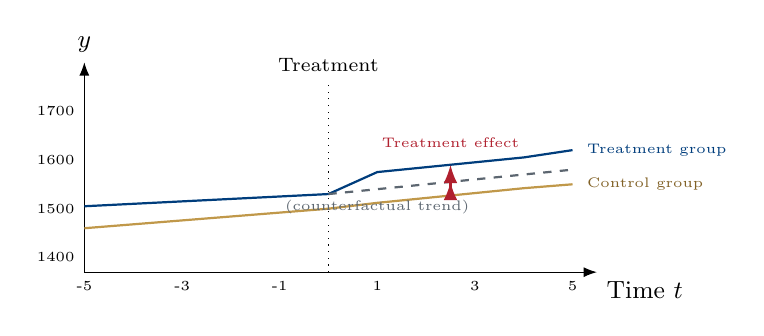
\begin{tikzpicture}[scale=0.62]
    \draw[-{Latex}] (0,-0.3) -- (10.5,-0.3) node[below right, font=\small]{Time $t$};
    \draw[-{Latex}] (0,-0.3) -- (0,4) node[above, font=\small]{$y$};
    \foreach \t/\lab in {0/-5,2/-3,4/-1,6/1,8/3,10/5}
      \node[below, font=\tiny] at (\t,-0.3) {\lab};
    \foreach \val/\lab in {0/1400,1/1500,2/1600,3/1700}
      \node[left, font=\tiny] at (0,\val) {\lab};
    \draw[dotted] (5,-0.3) -- (5,3.6);
    \node[above, font=\scriptsize] at (5,3.6) {Treatment};
    % treatment group: always visible
    \draw[wublue, thick] plot coordinates {(0,1.05) (1,1.10) (2,1.15) (3,1.20) (4,1.25) (5,1.30) (6,1.75) (7,1.85) (8,1.95) (9,2.05) (10,2.20)};
    \node[right, font=\tiny, wublue] at (10.1,2.20) {Treatment group};
    % control group (stage 2+)
    \onslide<2->{
      \draw[wuyellow!80!wugray, thick] plot coordinates {(0,0.60) (1,0.68) (2,0.76) (3,0.84) (4,0.92) (5,1.00) (6,1.12) (7,1.22) (8,1.32) (9,1.42) (10,1.50)};
      \node[right, font=\tiny, wuyellow!60!black] at (10.1,1.50) {Control group};
    }
    % counterfactual (stage 3+): treatment pre-level + control's post-treatment growth
    \onslide<3->{
      \draw[wugray, thick, dashed] (5,1.30) -- (10,1.80);
      \node[below, font=\tiny, wugray] at (6.0,1.37) {(counterfactual trend)};
    }
    % treatment effect arrow (stage 4+)
    \onslide<4->{
      \draw[wured, thick, {Latex}-{Latex}] (7.5,1.55) -- (7.5,1.90);
      \node[above, font=\tiny, wured, align=center] at (7.5,2.05) {Treatment effect};
    }
  \end{tikzpicture}
\end{frame}

\begin{frame}{Difference-in-Differences}
  \begin{itemize}
    \item DD assumes that the control group's path \emph{is} the counterfactual trend for the treatment group.
    \item \textbf{Common trends assumption}: absent treatment, the treatment group would have moved on the \emph{same} path as the control group.
    \begin{itemize}
      \item Not testable, but plausible if trends are parallel \emph{before} the treatment.
    \end{itemize}
  \end{itemize}
\end{frame}

\begin{frame}{When DD Does \emph{Not} Work: Diverging Pre-Trends}
  \centering
  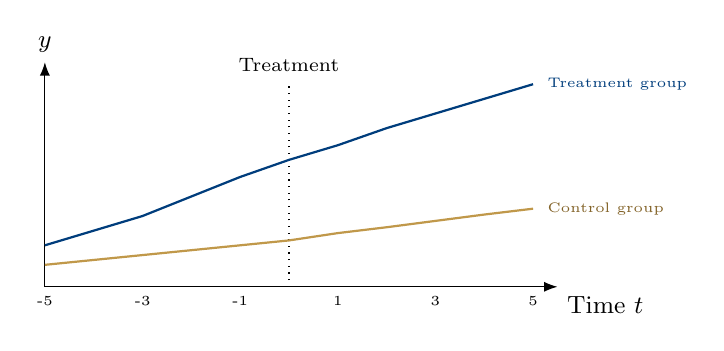
\begin{tikzpicture}[scale=0.62]
    \draw[-{Latex}] (0,-0.3) -- (10.5,-0.3) node[below right, font=\small]{Time $t$};
    \draw[-{Latex}] (0,-0.3) -- (0,4.3) node[above, font=\small]{$y$};
    \foreach \t/\lab in {0/-5,2/-3,4/-1,6/1,8/3,10/5}
      \node[below, font=\tiny] at (\t,-0.3) {\lab};
    \draw[dotted] (5,-0.3) -- (5,3.9);
    \node[above, font=\scriptsize] at (5,3.9) {Treatment};
    \draw[wublue, thick] plot coordinates {(0,0.55) (1,0.85) (2,1.15) (3,1.55) (4,1.95) (5,2.30) (6,2.60) (7,2.95) (8,3.25) (9,3.55) (10,3.85)};
    \node[right, font=\tiny, wublue] at (10.1,3.85) {Treatment group};
    \draw[wuyellow!80!wugray, thick] plot coordinates {(0,0.15) (1,0.25) (2,0.35) (3,0.45) (4,0.55) (5,0.65) (6,0.80) (7,0.92) (8,1.05) (9,1.18) (10,1.30)};
    \node[right, font=\tiny, wuyellow!60!black] at (10.1,1.30) {Control group};
  \end{tikzpicture}
  \vspace{0.3em}
  \footnotesize $\Rightarrow$ A DD estimate would \textbf{not} be credible here, because the treatment group is already rising much faster than the control group \emph{before} the treatment (no parallel trends).
\end{frame}

\begin{frame}{When DD Does \emph{Not} Work: Non-Parallel (Crossing) Trends}
  \centering
  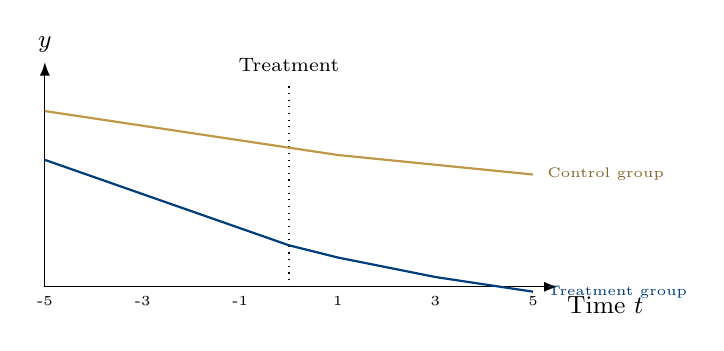
\begin{tikzpicture}[scale=0.62]
    \draw[-{Latex}] (0,-0.3) -- (10.5,-0.3) node[below right, font=\small]{Time $t$};
    \draw[-{Latex}] (0,-0.3) -- (0,4.3) node[above, font=\small]{$y$};
    \foreach \t/\lab in {0/-5,2/-3,4/-1,6/1,8/3,10/5}
      \node[below, font=\tiny] at (\t,-0.3) {\lab};
    \draw[dotted] (5,-0.3) -- (5,3.9);
    \node[above, font=\scriptsize] at (5,3.9) {Treatment};
    \draw[wuyellow!80!wugray, thick] plot coordinates {(0,3.3) (1,3.15) (2,3.0) (3,2.85) (4,2.7) (5,2.55) (6,2.4) (7,2.3) (8,2.2) (9,2.1) (10,2.0)};
    \node[right, font=\tiny, wuyellow!60!black] at (10.1,2.0) {Control group};
    \draw[wublue, thick] plot coordinates {(0,2.3) (1,1.95) (2,1.6) (3,1.25) (4,0.9) (5,0.55) (6,0.3) (7,0.1) (8,-0.1) (9,-0.25) (10,-0.4)};
    \node[right, font=\tiny, wublue] at (10.1,-0.4) {Treatment group};
  \end{tikzpicture}
  \vspace{0.3em}
  \footnotesize $\Rightarrow$ A DD estimate would also \textbf{not} be possible here, because the pre-treatment trends are not parallel (they cross).
\end{frame}

\begin{frame}{Difference-in-Differences}
  Under the common trends assumption, the treatment effect can be estimated with the following OLS regression:
  \[
    y_{it} = \beta_0 + \beta_1\, treated_i + \beta_2\, post_{it} + \delta\,(treated_i \times post_{it}) + \varepsilon_{it} \tag{4}
  \]
  \begin{itemize}
    \item $treated_i$ is a dummy indicating whether an observation is in the treatment ($treated_i = 1$) or control group ($treated_i = 0$).
    \item In the simplest case, $\hat\delta$ is the estimated difference in post-treatment means between the treatment and control group, net of the time-constant difference in $y$ between the two groups.
  \end{itemize}
\end{frame}

\begin{frame}{Difference-in-Differences}
  And to get dynamic effects:
  \[
    y_{it} = \beta_0 + \beta_1\, treated_i + \sum_{j=-5 \,|\, j\neq 0}^{5} \tau_j t_{ij} + \sum_{k=-5 \,|\, k\neq 0}^{5} \delta_k (treated_i \times t_{ik}) + \varepsilon_{it} \tag{5}
  \]
  \begin{itemize}
    \item The coefficients $\hat\delta_k$ measure the difference between the treatment and control group in each period $k$, relative to their difference in period 0.
  \end{itemize}
\end{frame}

\begin{frame}[fragile]
  \frametitle{Simulated Example: The Data}
{\tiny
\begin{verbatim}
. list id t post treated y in 1/22, sepby(id)

       id     t       post   treated         y

 1.     1    -5         0         0    1463.392
 2.     1    -4         0         0    1433.272
 3.     1    -3         0         0    1655.017
 4.     1    -2         0         0    1545.392
 5.     1    -1         0         0    1436.803
 6.     1     0         0         0    1556.735
 7.     1     1         1         0     1501.72
 8.     1     2         1         0    1612.518
 9.     1     3         1         0    1609.639
10.     1     4         1         0    1564.446
11.     1     5         1         0    1638.188

   [... id 2 (treated = 1) omitted here, same structure ...]
\end{verbatim}
}
\end{frame}

\begin{frame}[fragile]
  \frametitle{Simulated Example: Equation (4) by OLS}
{\scriptsize
\begin{verbatim}
. generate treatedXpost = treated*post
. reg y treated post treatedXpost
      Source         SS           df              MS        Number of obs    =    11,000
                                                             F(3, 10996)      =   1747.29
       Model     35405865.2            3     11801955.1     Prob > F         =    0.0000
    Residual     74271885.9       10,996     6754.44578     R-squared        =    0.3228
                                                             Adj R-squared    =    0.3226
       Total         109677751     10,999     9971.61115     Root MSE        =    82.185

               y            Coef.    Std. Err.        t       P>|t|       [95% Conf. Interval]

         treated         56.17291    2.122019      26.47      0.000       52.01337       60.33245
            post         73.14872    2.225592      32.87      0.000       68.78616       77.51128
    treatedXpost           30.436    3.147463       9.67      0.000       24.26641       36.60559
           _cons         1488.703    1.500494     992.14      0.000       1485.762       1491.644
\end{verbatim}
}
\vspace{0.3em}
$\Rightarrow$ How should the constant and the coefficients on \texttt{treated} and \texttt{post} be interpreted?\\
$\Rightarrow$ The estimated treatment effect is \textbf{30.4}.
\end{frame}

\begin{frame}[fragile]
  \frametitle{Simulated Example: Equation (5) by OLS}
{\tiny
\begin{verbatim}
. g t100 = t+100
. reg y b100.t100##i.treated
      Number of obs = 11,000    F(21, 10978) = 288.32    R-squared = 0.3555

           y       Coef.    Std. Err.        t       P>|t|    [95% Conf. Interval]

        t100
         95    -51.37909    5.075141     -10.12      0.000   -61.32729        -41.4309
         99    -2.968469    5.075141      -0.58      0.559   -12.91666        6.979722
   [...]
        101     30.71617    5.075141       6.05      0.000    20.76798        40.66437
        105      70.0025    5.075141      13.79      0.000    60.05431        79.95069

   1.treated    61.19874    5.075141      12.06      0.000    51.25054        71.14693

t100#treated
       95 1    -5.590081    7.177334      -0.78      0.436   -19.65895        8.478786
       99 1     -6.15418    7.177334      -0.86      0.391   -20.22305        7.914687
   [...]
      101 1     22.86918    7.177334       3.19      0.001    8.800316        36.93805
      105 1     29.53941    7.177334       4.12      0.000    15.47054        43.60827

       _cons    1512.386    3.588667     421.43      0.000    1505.351         1519.42
\end{verbatim}
}
\end{frame}

\begin{frame}{The Dynamic Interaction Coefficients, Plotted}
  \centering
  \begin{tikzpicture}[scale=0.62]
    \draw[-{Latex}] (0,1.0) -- (10.5,1.0) node[below right, font=\small]{Time $t$};
    \draw[-{Latex}] (0,-1.6) -- (0,3.4) node[above, font=\small]{OLS estimate};
    \foreach \t/\lab in {0/-5,2/-3,4/-1,6/1,8/3,10/5}
      \node[below, font=\tiny] at (\t,1.0) {\lab};
    \foreach \val/\lab in {-1.5/-30,-1.0/-10,1.5/10,2.5/30,3.4/50}
      \node[left, font=\tiny] at (0,\val) {\lab};
    \foreach \x/\y in {0/-0.56, 2/-1.04, 4/0.22, 6/-1.02, 8/-0.62}
      \fill[wublue] (\x,\y) circle (2.2pt);
    \fill[wublue] (5,1.0) circle (2.2pt);
    \foreach \x/\y in {6/2.29, 7/2.16, 8/2.43, 9/2.87, 10/2.95}
      \fill[wured] (\x,\y) circle (2.2pt);
  \end{tikzpicture}
  \vspace{0.3em}
  \footnotesize Coefficients on $treated_i \times t_{ik}$ from the regression above: flat and insignificant before treatment, positive and significant after.
\end{frame}

\begin{frame}{Difference-in-Differences}
  \framesubtitle{Example 1: Breast Cancer}
  \begin{itemize}
    \item \textbf{Ahammer, Pruckner \& Stiftinger (202x)}
    \item Breast cancer $\Longrightarrow$ health care spending, employment, wages
    \item Breast cancer = shock; women without breast cancer serve as the control group
    \begin{itemize}
      \item The control group receives a placebo shock based on the age-pdf
    \end{itemize}
    \item Model:
  \end{itemize}
  \[
    y_{it} = \beta_0 + \beta_1\, breastcancer_i + \sum_{j=-20 \,|\, j\neq -1}^{20} \tau_j t_{ij} + \sum_{k=-20 \,|\, k\neq -1}^{20} \delta_k (breastcancer_i \times t_{ik}) + \varepsilon_{it} \tag{6}
  \]
\end{frame}

\begin{frame}{Breast Cancer and Health Care Expenditures}
  \figplaceholder{11}{5.3}{Ahammer, Pruckner \& Stiftinger: level and change in healthcare expenditures, quarters relative to first (placebo) diagnosis, breast cancer patients vs.\ other women}
\end{frame}

\begin{frame}{Breast Cancer and Employment}
  \figplaceholder{11}{5.3}{Ahammer, Pruckner \& Stiftinger: level and change in days employed, quarters relative to first (placebo) diagnosis, breast cancer patients vs.\ other women}
\end{frame}

\begin{frame}{Breast Cancer and Wages}
  \figplaceholder{11}{5.3}{Ahammer, Pruckner \& Stiftinger: annual wage conditional on working and change in annual wage, quarters relative to first (placebo) diagnosis}
\end{frame}

\begin{frame}{Difference-in-Differences}
  \framesubtitle{Example 2: The ACA and Mortality}
  \begin{itemize}
    \item \textbf{Miller, Johnson \& Wherry (2021)}
    \item Affordable Care Act / Medicaid expansion $\Longrightarrow$ mortality?
    \item (Lack of) health insurance is a major issue in the US --- did Obamacare (= ACA) help?
    \item Expansion did not happen simultaneously in all states; states that had not yet expanded serve as the control group.
    \item Model:
  \end{itemize}
  \[
    mortality_{it} = \beta_0 + \beta_1\, statetreated_i + \sum_{j=-6\,|\,j\neq 0}^{3} \tau_j t_{ij} + \sum_{k=-6\,|\,k\neq 0}^{3} \delta_k (statetreated_i \times t_{ik}) + \varepsilon_{it} \tag{7}
  \]
\end{frame}

\begin{frame}{Mortality: States With vs.\ Without ACA Expansion}
  \figplaceholder{10.5}{5.3}{Miller, Johnson \& Wherry (2021) --- event-study coefficient plot, mortality by years relative to ACA/Medicaid expansion, states with vs.\ without expansion}
  \srcnote{Miller, Johnson \& Wherry (2021), \emph{Review of Economics and Statistics} 103(3).}
\end{frame}

\begin{frame}
  \centering
  \figplaceholder{9}{5.0}{(Optional) ``mic drop'' photo used here in the original slides as a punchline after the ACA mortality result}
\end{frame}

\begin{frame}{Difference-in-Differences}
  \framesubtitle{Example 3: Marijuana Legalization}
  \begin{itemize}
    \item \textbf{Wen, Hockenberry \& Cummings (2015)}
    \item Medical marijuana laws (MMLs); the gradual legalization of marijuana use for medical purposes in the US.
    \item How does legalization affect marijuana use among young people?
    \item States without MMLs serve as the control group.
  \end{itemize}
\end{frame}

\begin{frame}{Effect of Medical Marijuana Laws on Past-Month Use}
  \figplaceholder{11}{5.3}{Wen, Hockenberry \& Cummings (2015) --- \% difference in past-month marijuana use, months until/since the effective date of MMLs, by age group (12--20 and 21+)}
  \srcnote{Wen, Hockenberry \& Cummings (2015), \emph{NBER Working Paper} 20248.}
\end{frame}

% =============================================================
\section{Instrumental Variables}

\begin{frame}{Instrumental Variables}
  We are interested in the following model:
  \[
    y = \beta_0 + \beta_1 d + \varepsilon \tag{8}
  \]
  \begin{itemize}
    \item But we know the relationship is not causal, e.g.\ because of unobservable third variables or reverse causality.
    \item In an RCT, we would randomize $d$ and thereby estimate a causal effect.
    \item \textbf{Idea of an instrumental variable}: we look for a variable that performs this randomization for us.
  \end{itemize}
\end{frame}

\begin{frame}{Instrumental Variables}
  \centering
  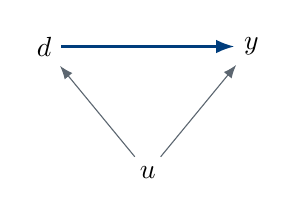
\begin{tikzpicture}[scale=1.0, node distance=2.2cm, every node/.style={font=\normalsize}]
    \node (d) {$d$};
    \node (y) [right=of d] {$y$};
    \node (u) [below=1.4cm of $(d)!0.5!(y)$] {$u$};
    \draw[-{Latex}, wublue, thick] (d) -- (y);
    \draw[-{Latex}, wugray] (u) -- (d);
    \draw[-{Latex}, wugray] (u) -- (y);
  \end{tikzpicture}
  \vspace{0.3em}
  \footnotesize An unobserved variable $u$ confounds both $d$ and $y$ --- the OLS estimate of $d \to y$ is biased.
\end{frame}

\begin{frame}{Instrumental Variables}
  \centering
  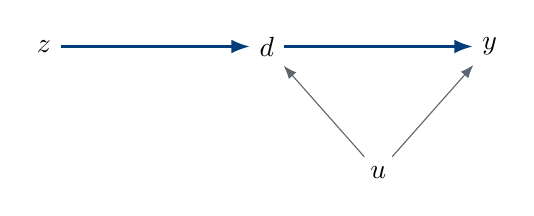
\begin{tikzpicture}[scale=1.0, node distance=2.4cm, every node/.style={font=\normalsize}]
    \node (z) {$z$};
    \node (d) [right=of z] {$d$};
    \node (y) [right=of d] {$y$};
    \node (u) [below=1.4cm of $(d)!0.5!(y)$] {$u$};
    \draw[-{Latex}, wublue, thick] (z) -- (d);
    \draw[-{Latex}, wublue, thick] (d) -- (y);
    \draw[-{Latex}, wugray] (u) -- (d);
    \draw[-{Latex}, wugray] (u) -- (y);
  \end{tikzpicture}
  \vspace{0.5em}
  \begin{itemize}
    \item $z$ is an \textbf{instrumental variable}.
    \item We can identify the effect of $d$ on $y$ caused by $z$, without controlling for $u$.
    \item \textbf{Most important assumption}: there is no direct effect $z \to y$ that does not run through $d$ (\textbf{exclusion restriction}).
  \end{itemize}
\end{frame}

\begin{frame}{Instrumental Variables}
  \framesubtitle{Example 1: Returns to Education}
  \begin{itemize}
    \item \textbf{Angrist \& Krueger (1991)}
    \item Returns to schooling: a causal effect is hard to estimate because the schooling decision is endogenous.
    \item Compulsory schooling duration $\to$ schooling decision $\to$ income.
    \item Changes in compulsory schooling duration: birth date (quasi-random!) determines whether one can leave school at 15 or 16.
    \item The design estimates the effect of additional schooling induced by an increase in compulsory schooling duration (external validity).
  \end{itemize}
\end{frame}

\begin{frame}{Instrumental Variables}
  \framesubtitle{Example 2: Judge Assignment}
  \begin{itemize}
    \item \textbf{Aizer \& Doyle Jr.\ (2015)}
    \item How does incarceration affect recidivism?
    \item Judge strictness $\to$ incarceration $\to$ probability of reoffending.
    \item Random assignment to judges in the US --- some are stricter than others.
    \item The design estimates the effect of \emph{marginal} incarceration: what is the recidivism rate among people who end up incarcerated only because they happened to draw a strict judge?
  \end{itemize}
\end{frame}

\begin{frame}{Instrumental Variables}
  Estimation using a two-stage model (two-stage least squares, 2SLS):
  \begin{enumerate}
    \item \textbf{First stage}:
    \[
      d_i = \alpha_0 + \alpha_1 z_i + \xi_i \tag{9}
    \]
    \item Compute the fitted value $\hat d_i$ for all $i$.
    \item \textbf{Second stage}:
    \[
      y_i = \beta_0 + \beta_1 \hat d_i + \varepsilon_i \tag{10}
    \]
  \end{enumerate}
  \begin{itemize}
    \item Standard errors in the second stage must be adjusted, because $\hat d_i$ is itself estimated from the data.
    \item Identifies the so-called \textbf{local average treatment effect (LATE)}.
  \end{itemize}
\end{frame}

\begin{frame}[fragile]
  \frametitle{Simulated Example: First Stage}
{\scriptsize
\begin{verbatim}
. clear
. set obs 10000
number of observations (_N) was 0, now 10,000
. g z = rnormal(50, 10)
. g d = 5 + .5*z + rnormal(0, 1.5)
. g y = 2.5 + .25*d + rnormal(0, 2)
. reg d z
      Source         SS            df            MS        Number of obs    =     10,000
                                                            F(1, 9998)       >   99999.00
       Model     248031.051            1    248031.051     Prob > F         =     0.0000
    Residual     22959.4347        9,998    2.29640275     R-squared        =     0.9153
                                                            Adj R-squared    =     0.9153
       Total     270990.486        9,999    27.1017588     Root MSE         =     1.5154

           d           Coef.    Std. Err.        t       P>|t|       [95% Conf. Interval]

           z         .5009801   .0015244     328.65      0.000        .497992       .5039681
       _cons         4.954964   .0777234      63.75      0.000        4.80261       5.107317
\end{verbatim}
}
\end{frame}

\begin{frame}[fragile]
  \frametitle{Simulated Example: Naive Second Stage}
{\scriptsize
\begin{verbatim}
. predict d_hat, xb
. reg y d_hat
      Source            SS            df         MS       Number of obs    =     10,000
                                                           F(1, 9998)       =    3665.97
      Model      15115.1207            1    15115.1207    Prob > F         =     0.0000
   Residual      41222.6029        9,998    4.12308491    R-squared        =     0.2683
                                                           Adj R-squared    =     0.2682
      Total      56337.7236        9,999    5.6343358     Root MSE         =     2.0305

           y           Coef.    Std. Err.        t      P>|t|       [95% Conf. Interval]

      d_hat          .2468612   .0040772      60.55     0.000       .2388691       .2548532
      _cons          2.572058   .1240221      20.74     0.000       2.328949       2.815166
\end{verbatim}
}
\vspace{0.3em}
\footnotesize Note: the point estimate is correct, but the standard errors here are \emph{not} --- they need the 2SLS correction on the next slide.
\end{frame}

\begin{frame}[fragile]
  \frametitle{Simulated Example: Proper 2SLS}
{\tiny
\begin{verbatim}
. ivreg2 y (d=z)
IV (2SLS) estimation                            Number of obs = 10000   F(1,9998) = 3801.35

           y           Coef.     Std. Err.       z    P>|z|       [95% Conf. Interval]

          d          .2468612   .0040035      61.66   0.000       .2390144      .2547079
      _cons          2.572058   .1217816      21.12   0.000        2.33337      2.810745

Underidentification test (Anderson canon. corr. LM statistic):                  9152.759
                                                   Chi-sq(1) P-val =              0.0000

Weak identification test (Cragg-Donald Wald F statistic):                        1.1e+05
Stock-Yogo weak ID test critical values: 10% maximal IV size                       16.38

Instrumented:         d
Excluded instruments: z
\end{verbatim}
}
\end{frame}

% =============================================================
\section{Regression Discontinuity Design}

\begin{frame}{Regression Discontinuity Design}
  \begin{itemize}
    \item \textbf{Setting}: treatment is assigned via a cutoff.
    \begin{itemize}
      \item Unemployed workers over 40 receive unemployment benefits for longer.
      \item Students with an ACT score above 35 are admitted to Harvard.
      \item Newborns weighing less than 2{,}500g receive special treatment.
    \end{itemize}
    \item \textbf{Idea}: observations in a very small window around the cutoff (= \textbf{bandwidth}) are as good as randomly assigned.
    \begin{itemize}
      \item You cannot choose whether you become unemployed at age 39.9 or 41.1.
      \item It is quasi-random whether you score 34.9 or 35 on the ACT.
      \item It is quasi-random whether birth weight is 2{,}499g or 2{,}500g.
    \end{itemize}
    \item \textbf{Most important assumption}: you cannot choose whether you fall above or below the cutoff (\textbf{no manipulation assumption}).
    \item A \emph{local} experiment.
  \end{itemize}
\end{frame}

\begin{frame}{Regression Discontinuity Design}
  \centering
  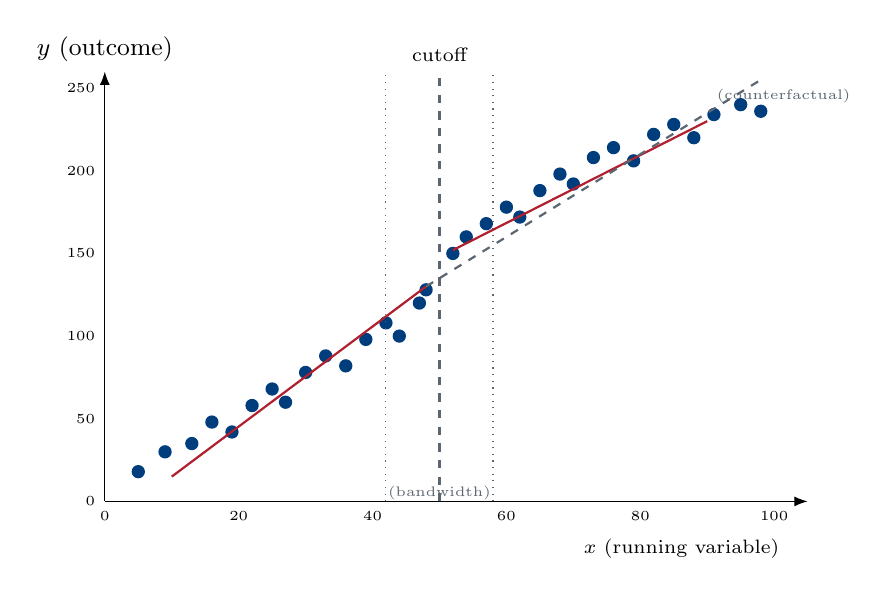
\begin{tikzpicture}[xscale=0.085, yscale=0.021]
    \draw[-{Latex}] (0,0) -- (105,0) node[below, font=\scriptsize, xshift=-1.6cm, yshift=-0.35cm]{$x$ (running variable)};
    \draw[-{Latex}] (0,0) -- (0,260) node[above, font=\small]{$y$ (outcome)};
    \foreach \x in {0,20,40,60,80,100}
      \node[below, font=\tiny] at (\x,0) {\x};
    \foreach \y in {0,50,100,150,200,250}
      \node[left, font=\tiny] at (0,\y) {\y};
    % scatter: left cloud
    \foreach \x/\y in {5/18,9/30,13/35,16/48,19/42,22/58,25/68,27/60,30/78,33/88,36/82,39/98,42/108,44/100,47/120,48/128}
      \node[circle, fill=wublue, inner sep=1.7pt] at (\x,\y) {};
    % scatter: right cloud
    \foreach \x/\y in {52/150,54/160,57/168,60/178,62/172,65/188,68/198,70/192,73/208,76/214,79/206,82/222,85/228,88/220,91/234,95/240,98/236}
      \node[circle, fill=wublue, inner sep=1.7pt] at (\x,\y) {};
    \onslide<2->{
      \draw[wugray, dashed, thick] (50,0) -- (50,260);
      \node[above, font=\scriptsize] at (50,260) {cutoff};
      \draw[wugray, dotted] (42,0) -- (42,260);
      \draw[wugray, dotted] (58,0) -- (58,260);
      \node[below, font=\tiny, wugray] at (50,15) {(bandwidth)};
    }
    \onslide<3->{
      \draw[wured, thick] (10,15) -- (48,130);
      \draw[wured, thick] (52,152) -- (90,230);
    }
    \onslide<4->{
      \draw[wugray, thick, dashed] (48,130) -- (98,255);
      \node[right, font=\tiny, wugray] at (90,245) {(counterfactual)};
    }
  \end{tikzpicture}
\end{frame}

\begin{frame}{Regression Discontinuity Design}
  Estimation is possible with OLS:
  \[
    y_i = \beta_0 + \beta_1 (x_i - c_0) + \delta d_i + \varepsilon_i \tag{11}
  \]
  where $c_0$ is the cutoff (50 in the previous example) and $d_i = \mathbf{1}\{x_i > c_0\}$.
  \vspace{0.3em}

  \textbf{Modeling decisions}:
  \begin{itemize}
    \item \textbf{Bandwidth} (the smaller, the ``better'' the local experiment --- but the higher the data requirement)
    \item \textbf{Bin size} (the $x$-axis is typically ``binned'')
    \item \textbf{Trends} (the running variable is modeled linearly here; a higher-order polynomial may be necessary)
  \end{itemize}
  \vspace{0.3em}
  \textbf{Validity tests}: are covariates ``smooth'' around the cutoff? Is there ``bunching'' at or below the cutoff?
  \vspace{0.3em}

  $\delta$ is again a local average treatment effect.
\end{frame}

\begin{frame}{Regression Discontinuity Design}
  \framesubtitle{Example: The Effect of Unemployment Benefits}
  \begin{itemize}
    \item \textbf{Nekoei \& Weber (2009)}
    \item Unemployment benefits are extended by 9 weeks if the worker is $\geq 40$ years old and worked in 6 of the last 10 years.
    \item \textbf{Mechanism}: signalling vs.\ more time to search for better jobs.
    \item Effects on labor-market outcomes.
    \item \textbf{Extension}: effects on health (Ahammer \& Packham 2023).
  \end{itemize}
\end{frame}

\begin{frame}{Validity Check: Distribution of Age at Layoff}
  \figplaceholder{10}{4.8}{Nekoei \& Weber (2009), Panel A --- density of age at layoff around the age-40 cutoff (smoothness/no-manipulation check)}
\end{frame}

\begin{frame}{Validity Check: Covariates Around the Cutoff}
  \figplaceholder{10}{4.8}{Nekoei \& Weber (2009), Panel B --- log previous wage by age at layoff around the UI-extension cutoff}
\end{frame}

\begin{frame}{Main Results: Labor-Market Outcomes}
  \figplaceholder{11}{5.3}{Nekoei \& Weber (2009) --- four-panel RDD results: nonemployment duration, probability of finding a job within 39 weeks, wage change between jobs, and new wage $>$ 0.5 $\times$ old wage, all vs.\ age at layoff}
\end{frame}

\begin{frame}{Main Results: Regression Table}
  \figplaceholder{11}{4.7}{Nekoei \& Weber (2009), Table 2 --- ``Effect of UI Benefit Extension from 30 to 39 Weeks''}
  \srcnote{Nekoei \& Weber (2009/2017), \emph{American Economic Review} 107(2).}
\end{frame}

\begin{frame}{Extension: Effects on Mental Health}
  \figplaceholder{10.5}{5.0}{Ahammer \& Packham (2023), Figure 7 --- effects of extended UI benefit duration on the probability of being prescribed drugs for depression, by sex, age at start of unemployment}
  \srcnote{Ahammer \& Packham (2023).}
\end{frame}

% =============================================================
\begin{frame}[standout]
  Any questions?\\[0.5em]
  {\small \figplaceholder{6}{3.2}{(Optional) humorous image used here in the original slides}}
\end{frame}

\end{document}
